\section{Building Blocks}\label{section:building-blocks}

As depicted in Figure~\ref{figure:building-blocks}, our solution is composed of a three-tiered web application based on Ruby on Rails\foo{http://rubyonrails.org/}, and a Docker server. The web application provides the development environment for learners as well as an administration back-end for teachers. Docker is used for code execution and assessment. Both core components can either be located on the same host or on different ones.

The web application communicates with the Docker server using its \gls{http}-based Remote \gls{api}\foo{https://docs.docker.com/reference/api/docker_remote_api/}. For this purpose, it utilizes an object-oriented interface to the \gls{api}, which is provided by the docker-api\foo{https://github.com/swipely/docker-api} Ruby package, a so-called gem.

\begin{figure}
\centering
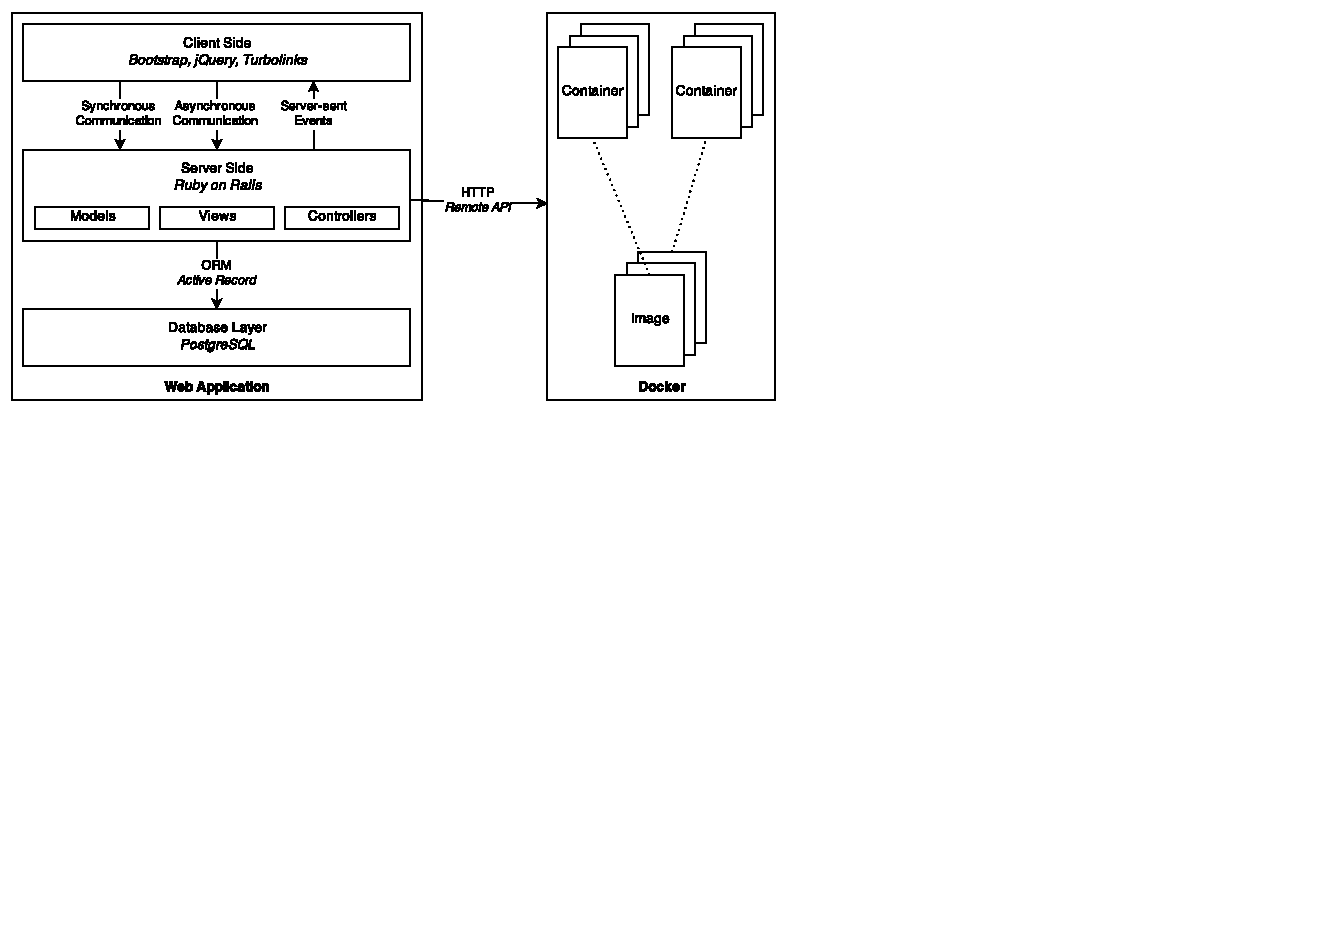
\includegraphics[clip=true, trim=0.1cm 9.2cm 9.4cm 0.2cm, width=\textwidth]{images/building-blocks.pdf}
\caption{Building Blocks of \tool}
\label{figure:building-blocks}
\end{figure}

\paragraph{Client Side}

\tool's client-side portion is built using the open-source front-end framework Bootstrap\foo{http://getbootstrap.com/} and the open-source library jQuery\foo{http://jquery.com/}, which facilitate the construction of a visually pleasing \gls{ui} that is cross-browser compatible and compliant to modern web standards. The \gls{ui}'s responsive layout provides proper usability on various client platforms, including mobile devices.

Client-server communication is heavily based on \gls{ajax}. Asynchronous background requests enable a single-page development workflow for the web-based development environment. Moreover, Rails' Turbolinks\foo{https://rubygems.org/gems/turbolinks} feature improves page load times when navigating through the application by partially reloading visible content instead of performing full page loads.

\paragraph{Server Side}

Based on positive experience and due to its reputation as a highly productive web framework~\cite{fox2012crossing}, we decided in favor of Rails. Rails produces reliable, concise code~\cite{geer2006will}, not least due to the flexibility of Ruby, its underlying programming language. By favoring convention over configuration and promoting built-in automated testing, Ruby on Rails facilitates the development of powerful web applications.

As provided by Rails, \tool's server-side code is organized according to the \gls{mvc} architectural pattern~\cite{krasner1988description}.

\paragraph{Database}

In consequence of positive experience with PostgreSQL\foo{http://www.postgresql.org/}, \tool has been developed and deployed using this database technology. However, thanks to Active Record\foo{https://rubygems.org/gems/activerecord}, which is Rails' database-agnostic \gls{orm} component and an implementation of the same-titled design pattern~\cite{fowler2002patterns}, the application's underlying database is easily exchangeable if desired.
